\documentclass{jknotes}
\usepackage{../joshkirklin}

\setmathfont{Latin Modern Math}
\setmathfont{GFS NeoHellenic Math}[range=bfsfup/{greek,Greek}->it]
\setmathfont{GFS NeoHellenic Math}[range=sfup/{latin,Latin}->it]

\usetikzlibrary{shapes.misc}

\tikzset{cross/.style={cross out, draw=black, minimum
size=2*(#1-\pgflinewidth), inner sep=0pt, outer sep=0pt}}
%default radius will be 1pt. 

\newcommand{\myol}[2][3]{{}\mkern#1mu\overline{\mkern-#1mu#2}}

\begin{document}

\institution{Cambridge Part III Maths}
\title{Fluid Dynamics of Environment}
\lecturer{Dr. Stuart Dalziel}
\notetaker{Charles Powell}
\date{Lent 2020}

\maketitle
\suggestionsspiel
\tableofcontents

\lecture{22/01/21}
\section{Internal waves}

\subsection{Intuitive version}

\begin{center}
	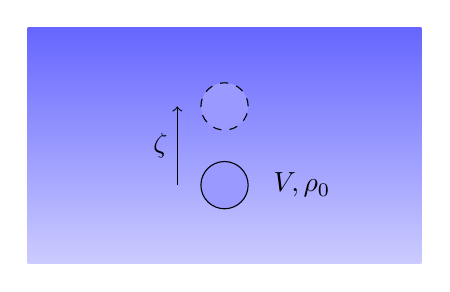
\begin{tikzpicture}
		\draw[draw=none,top color = blue!60, bottom color = blue!20] (0,0) rectangle (5, 3);
		\draw[fill=blue!40] (2.5, 1) circle (0.3);
		\draw (3, 1) node[right] {$V, \rho_0$};
		\draw[dashed,fill=blue!40] (2.5, 2) circle (0.3);
		\draw[->] (1.9, 1) -- (1.9, 2) node[midway,left] {$\zeta$};
	\end{tikzpicture}
\end{center}
Consider a fluid parcel of volume $V$ and density $\rho_0$ in a fluid with
density profile $\hat{\rho}(z)$.  Suppose the parcel is moved upwards by
$\zeta$. The parcel experiences a \emph{buoyancy force} $B = g V \zeta
\frac{\diffd \hat{\rho}}{\diffd z}$. Newton's second law gives
\begin{equation}
	\ddot{\zeta} + \left(-\frac{g}{\rho_0} \frac{\diffd \hat{\rho}}{\diffd
	z}\right) \zeta = 0
\end{equation}
The \emph{buoyancy frequency} (or Brunt-V\"{a}is\"{a}l\"{a} frequency) is
defined as 
\begin{equation}
	N^2 = - \frac{g}{\rho} \frac{\diffd \hat{\rho}}{\diffd z}
\end{equation}
which has general solution
\begin{equation}
	\zeta = A \cos N t + B \sin N t
\end{equation}
If we instead consider a fluid slab inclined at angle $\theta$ with the
vertical rather than a fluid parcel, the slab can fall in its plane much more
easily than in the vertical. Hence in this situation we have
\begin{equation}
	\ddot{\zeta} + N^2 \cos^2\theta \zeta = 0
\end{equation}
The dispersion relation is thus $\omega/N = \cos \theta$.

Now consider a sphere oscillating at frequency $\omega$ in the vertical in a
stratified fluid with density $\rho(z)$. The fluid resonates in bands at angle
$\theta$ satisfying the dispersion relation, provided $\omega < N$.
Intuitively, the group velocity must be out of the beams as energy is radiated
away.
\begin{center}
	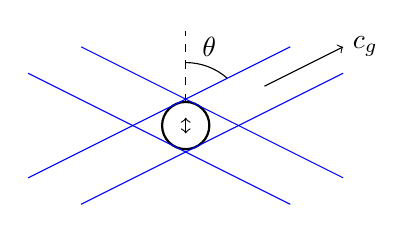
\begin{tikzpicture}
		\draw[thick] (0,0) circle (0.3);
		\draw[<->] (0, 0.1) -- (0, -0.1);
		\draw[blue] (1.328,1) -- (-2, -0.664);
		\draw[blue] (-1.328,-1) -- (2, 0.664);
		\draw[blue] (-1.328,1) -- (2, -0.664);
		\draw[blue] (1.328,-1) -- (-2, 0.664);
		\draw[dashed] (0, 0.3) -- (0, 1.2);
		\draw (0,0.8) arc (90:49:0.8);
		\draw (0.3, 1) node {$\theta$};
		\draw[->] (1, 0.5) -- (2,1) node[right] {$\symbf{c}_g$};
	\end{tikzpicture}
\end{center}

At the leading edge of the rays, baroclinic vorticity is generated by the
movement of fluid of different density to its surroundings. This provides the
mechanism for the instability.

\subsection{Rigorous derivation}
Consider a fluid in which the mean pressure $p_0(z)$ and the mean density
$\rho_0(z)$ are in hydrostatic balance when the fluid is at rest:
\begin{equation}
	\frac{\diffd p_0}{\diffd z} = - \rho_0 g
\end{equation}

Assume that the vertical lengthscale for $\rho_0$ variation is $L$. Motion is
governed by the Navier-Stokes equations \eqref{eq:incomp} and \eqref{eq:ns} with
$\nu = 0$, and mass conservation \eqref{eq:masscons}. 
\begin{align}
	\nabla \cdot \symbf{u} &= 0 \label{eq:incomp} \\
	\rho \frac{\partial \symbf{u}}{\partial t} + \rho
	(\symbf{u}\cdot\nabla)\symbf{u} &= - \nabla p - \rho g \hat{\symbf{z}}
	\label{eq:ns} \\
	\left(\frac{\partial}{\partial t} + \symbf{u}\cdot \nabla \right) \rho = 0
	\label{eq:masscons}
\end{align}

Following the Boussinesq approximation, assume small perturbations to the mean
state: $\rho = \rho_0(z) + \tilde{\rho}$ and $p = p_0(z) + \tilde{p}$ where
$\tilde{p} \ll p_0, \tilde{\rho} \ll \rho_0$. Under this approximation, the
momentum equation \eqref{eq:ns} becomes
\begin{align}
	\frac{\partial \symbf{u}}{\partial t} + (\symbf{u}\cdot\nabla)\symbf{u} 
	&= - \frac{1}{\rho_0}\nabla p - \frac{\rho}{\rho_0} g \hat{\symbf{z}} \\ 
	&= - \frac{1}{\rho_0} \nabla(p + \rho_0 g z) - g' \hat{\symbf{z}}
\end{align}
where $g' = g(\rho-\rho_0)/\rho_0$ is the \emph{reduced gravity}. We now
linearise $\symbf{u}$ about a state of rest, ignoring second order quantities
in the velocity disturbance $\symbf{u}'$. It is now further desirable to split
the disturbance components into $\tilde{\rho} = \hat{\rho} + \rho', \tilde{p}
= \hat{p} + p'$ where $\hat{\rho}, \hat{p}$ are in hydrostatic balance. We
have
\begin{align}
	\nabla \cdot \symbf{u}' &= 0  \\
	\frac{\partial \rho'}{\partial t} + w' \frac{\diffd \hat{\rho}}{\diffd z}
							&= \frac{\partial \rho'}{\partial t} - w' \frac{\rho_0}{g}N^2 
							= 0 \\
	\frac{\partial \symbf{u}'}{\partial t} 
							&= -\frac{1}{\rho_0}\nabla (p_0+\hat{p}) -
							\frac{g\hat{\rho}}{\rho_0}\hat{\symbf{z}} -
							\frac{1}{\rho_0} \nabla p' -
							\frac{g\rho'}{\rho_0}\hat{\symbf{z}}
							\label{eq:idk} 
\end{align}
Hydrostatic balance eliminates the first two RHS terms of the momentum
equation; the
hydrostatic pressure field is 
\begin{equation}
	p_0 + \hat{p} = -\int g \hat{\rho} \, \diffd z
\end{equation}
Finally we have
\begin{equation}
	\frac{\partial \symbf{u}'}{\partial t} = -\frac{1}{\rho_0} \nabla p' -
	\frac{g\rho'}{\rho_0} \hat{\symbf{z}}
\end{equation}
Define buoyancy $b = - g \rho'/\rho_0$. The governing equations are now
\begin{align}
	\frac{\partial b}{\partial t} &= -\frac{1}{\rho_0} \nabla p' + b
	\hat{\symbf{z}} \\
	\frac{\partial \symbf{u}'}{\partial t} &= -\frac{1}{\rho_0} \nabla p' + b
	\hat{\symbf{z}}
\end{align}
To eliminate pressure, we take the curl of the momentum equation to get
\begin{equation}
	\frac{\partial \symbf{\zeta}'}{\partial t} = -\hat{\symbf{z}}\times\nabla
	b
\end{equation}
where $\symbf{\zeta}' = \nabla \times \symbf{u}'$ is the disturbance
vorticity. Using the buoyancy equation we have
\begin{equation}
	\left[ \nabla^2 \frac{\partial^2}{\partial t^2} + N^2 \nabla_H^2\right] w'
	= 0
\end{equation}
where $\nabla_H = (\partial_x,\partial_y)$ is the horizontal gradient
operator. This equation admits plane wave solutions
\begin{equation}
	w'(\symbf{x},t) = \Re\left[ \hat{w}(t) e^{i(k_x x + k_y y - \omega
	t)}\right]
\end{equation}
where $\hat{w}$ satisfies
\begin{equation}
	\frac{\diffd^2 \hat{w}}{\diffd z^2} + (k_x^2 + k_y^2)(\frac{N^2}{\omega^2}
	- 1) \hat{w} = 0
\end{equation}
which has general solution
\begin{align}
	\hat{w} &= \Re\left[ A e^{-inz} + Be^{inz}\right] \\
	n^2 &= (k_x^2 + k_y^2)(\frac{N^2}{\omega^2} - 1)
\end{align}
If $\omega > N$, $n$ is imaginary and, defining $\gamma =
\sqrt{1-N^2/\omega^2}$, we have
\begin{equation}
	w' = (A e^{-\gamma k z} + B e^{\gamma kz}) e^{i(k_x x + k_y y - \omega
	t)}
\end{equation}
When $N = 0$, we get potential flow. If $0 < N < \omega$ then we have rescaled
potential flow, with scaling $\gamma$. If $\omega < N$ then $n$ is real and
solutions are oscillatory with
\begin{equation}
	n^2 = k z^2 = (k_x^2 + k_y^2)(\frac{N^2}{\omega^2} - 1)
\end{equation}
The wavenumber vector is $\symbf{k} = (k_x, k_y, k_z) = (k,l,m)$. Hence
\begin{equation}
	\frac{\omega^2}{N^2} = \frac{k_x^2 + k_y^2}{k_x^2+k_y^2+k_z^2} = 1 -
	\frac{k_z^2}{\abs{\symbf{k}}^2} = \cos^2 \theta
\end{equation}
where $\theta$ is the angle between $\symbf{k}$ and the horizontal plane. Note
that $N$ is assumed constant.

\begin{center}
	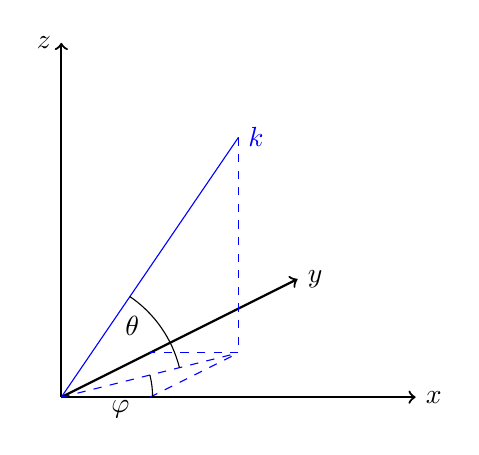
\begin{tikzpicture}[scale=1.5]
		\draw[thick,->] (0,0) -- (3, 0) node[right] {$x$};
		\draw[thick,->] (0,0) -- (0, 3) node[left] {$z$};
		\draw[thick,->] (0,0) -- (2, 1) node [right] {$y$};
		\draw[blue] (0,0) -- (1.5, 2.2) node [right] {$\symbf{k}$};
		\draw[blue,dashed] (1.5, 2.2) -- (1.5, 0.375);
		\draw[blue,dashed] (0,0) -- (1.5, 0.375);
		\draw[blue,dashed] (0.75,0) -- (1.5, 0.375);
		\draw[blue,dashed] (1.5, 0.375) -- (0.75,0.375);
		\draw (1,0.25) arc (14:55.7:1.03);
		\draw (0.75,0.1875) arc (14:0:0.77);
		\draw (0.5, -0.1) node {$\varphi$};
		\draw (0.6, 0.6) node {$\theta$};
	\end{tikzpicture}
\end{center}

We will use $\theta$ as the angle between the horizontal plane and
$\symbf{k}$, hence $\omega/N = \cos \theta$. Some authors use the polar
inclination angle between $\hat{\symbf{z}}$ and $\symbf{k}$, in which case
$\omega/N = \sin\theta$. The azimuthal angle between the $x$ axis and the
projection of $\symbf{k}$ onto the horizontal plane is denoted by $\varphi$.
We will also assume $\omega \ge 0$ going forward. The wavevector takes the
form
\begin{equation}
	\symbf{k} = \abs{\symbf{k}} \begin{pmatrix} \cos\varphi\cos\theta \\
	\sin\varphi\cos\theta \\ \sin \theta \end{pmatrix}
\end{equation}

The \emph{phase} of the wave is defined to be $\phi = \symbf{k}\cdot\symbf{x}
- \omega t$. Note the following:
\begin{align}
	e^{i\phi} &= e^{i(\symbf{k}\cdot\symbf{x}-\omega t)} \\
	\Re\left[ e^{i\phi}\right] &= \Re\left[ e^{-i\phi}\right] \\
	\Re\left[ \tilde{\eta}e^{i\phi}\right] &= \Re\left[\tilde{\eta}^*
	e^{-i\phi}\right]
\end{align}

We will focus on 2D waves. By suitable choice of coordinate system, 3D waves
can be reduced to 2D. In the (x,z) plane, from $\nabla \cdot \symbf{u} = 0$
and assuming $w(\symbf{x},t) = \tilde{w}e^{i\phi}$ with $\tilde{w} \in
\mathbb{C}$ we have
\begin{equation}
	u = \int -\frac{\partial w}{\partial z} \, \diffd x = -\frac{m}{k}
	\tilde{w}e^{i\phi} = - \tan \theta \tilde{w} e^{i\phi}
\end{equation}
\begin{center}
	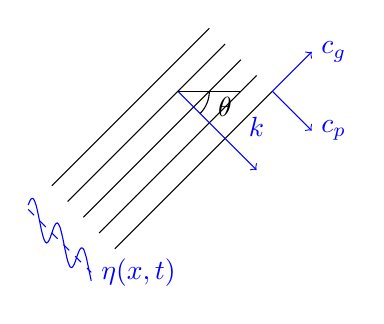
\begin{tikzpicture}
		\draw (0,0) -- ++ (2,2);
		\draw (0.2, -0.2) -- ++(2,2);
		\draw (0.4, -0.4) -- ++(2,2);
		\draw (0.6, -0.6) -- ++(2,2);
		\draw (0.8, -0.8) -- ++(2,2);
		\draw[blue,->] (1.6, 1.2) --++(1,-1);
		\draw[blue,dashed] (-0.3, -0.3) -- ++ (0.8, -0.8);
		\draw[smooth,blue] plot[domain=-0.3:0.5]
		({\x},{0.2*sin(20*deg(\x))-\x-0.6});
		\draw[blue] (1.1, -1.1) node {$\eta(\symbf{x},t)$};
		\draw[blue] (2.6, 0.75) node {$\symbf{k}$};
		\draw[blue,->] (2.8, 1.2) -- ++(0.5, -0.5) node [right] {$\symbf{c}_p$};
		\draw[blue,->] (2.8, 1.2) -- ++(0.5, 0.5) node [right] {$\symbf{c}_g$};
		\draw (1.6, 1.2) -- (2.4, 1.2);
		\draw (2,1.2) arc (0:-45:0.4);
		\draw (2.2, 1) node {$\theta$};
	\end{tikzpicture}
\end{center}
Denoting the wave displacement by $\eta(\symbf{x},t) = \tilde{\eta}e^{i\phi}$
we have the following:
\begin{align}
	\frac{\partial \eta}{\partial t} &= -i\omega \tilde{\eta} e^{i\phi} \\
	u(\symbf{x},t) &= \tilde{u}e^{i\phi} = -i\omega \sin\theta
	\tilde{\eta}e^{i\phi} \\
	w(\symbf{x},t) &= \tilde{w}e^{i\phi} = i\omega \cos\theta
	\tilde{\eta}e^{i\phi} \\
\end{align}

Using the buoyancy equation $\partial b / \partial t = - w N^2$ we also find
\begin{equation}
	i\omega \tilde{b} = - \tilde{w}N^2 \implies b = - \tilde{\eta}
	\frac{\omega^2}{\cos\theta} e^{i\phi} = - \tilde{\eta}\omega N e^{i\phi}
\end{equation}
Similarly the pressure field follows from the momentum equation
\begin{equation}
	\frac{\partial u}{\partial t} = - \frac{1}{\rho_0} \frac{\partial
	p'}{\partial x} \implies \tilde{p} = i\frac{\omega^2}{k}
	\tilde{\eta}\sin\theta
\end{equation}

\subsection{Wave velocities}
\subsubsection{Phase velocity}
For the phase $\phi =
\symbf{k}\cdot\symbf{x} - \omega t$ we can write
\begin{align}
	\frac{\partial \phi}{\partial x_i} \frac{\partial \phi}{\partial t} -
	\frac{\partial \phi}{\partial t} \frac{\partial \phi}{\partial x_i} &= 0
	\\
	\implies k_i \frac{\partial \phi}{\partial t} + \omega \frac{\partial
\phi}{\partial x_i} &= 0\\
\implies \frac{\partial \phi}{\partial t} + \frac{\omega}{\abs{\symbf{k}}^2}
k_i \frac{\partial \phi}{\partial x_i}
\end{align}
Defining the phase velocity $\symbf{c}_p = \frac{\omega}{\abs{\symbf{k}}^2}
\symbf{k}$ as the velocity at which the phase is advected, we have
\begin{equation}
	\frac{\partial \phi}{\partial t} + (\symbf{c}_p \cdot \nabla) \phi = 0
\end{equation}

For all waves, this is the speed at which wave crests move. For deep water
waves with dispersion relation $\omega = \sqrt{gk}$ we find $c_p =
\sqrt{g/k}$. 

\subsubsection{Group velocity}
By symmetry of partial differentiation, we may write
\begin{align}
	\frac{\partial^2 \phi}{\partial t \partial x_i} - 
	\frac{\partial^2 \phi}{\partial t \partial x_i} &= 0 \\
	\implies \frac{\partial k_i}{\partial t} + \frac{\partial \omega}{\partial
x_i} &= 0 \label{eq:132}
\end{align}
If $\omega = \omega(\symbf{k})$ then from chain rule
\begin{equation}
	\frac{\partial \omega}{\partial x_i} = \frac{\partial \omega}{\partial
	k_j} \frac{\partial k_j}{\partial x_i}
\end{equation}
We also know from definition of phase
\begin{equation}
	\frac{\partial k_j}{\partial x_i} = \frac{\partial}{\partial x_i} \left(
	\frac{\partial \phi}{\partial x_j} \right) = \frac{\partial k_i}{\partial
	x_j}
\end{equation}
Hence  \eqref{eq:132} may be written as
\begin{equation}
	\frac{\partial k_i}{\partial t} + \frac{\partial \omega}{\partial k_j}
	\frac{\partial k_i}{\partial x_j} = 0
\end{equation}
Thus we define the group velocity as the velocity at which the wavevector is
advected, i.e. $\symbf{c}_g = \frac{\partial \omega}{\partial k_i}$ and
\begin{equation}
	\left( \frac{\partial}{\partial t} + \symbf{c}_g \cdot \nabla \right)
	\symbf{k} = 0
\end{equation}
For deep water waves, we thus have $c_g = \sqrt{g/k}/2 = c_p/2$.
\subsubsection{Superposition}
Consider two waves with slightly different wavenumber and frequency
superposed:
\begin{align}
	\eta &= \cos \left( (k+\delta k)x - (\omega+\delta \omega)t\right) + \cos
	\left( (k-\delta k)x - (\omega - \delta\omega)t\right) \\
		 &= 2 \cos \left( \delta k x - \delta \omega t\right) \cos \left( kx -
		 \omega t\right)
\end{align}
This is referred to as \emph{modulation} with $\abs{\delta k} \ll \abs{k},
\abs{\delta \omega} \ll \abs{\omega}$. Equivalently, in the limit as
$\abs{\delta k} \to 0, \abs{\delta \omega} \to 0$, we have
\begin{equation}
	\eta = 2 \cos \left( (x-\frac{\partial \omega}{\partial k} t)\delta
	k\right)
	\cos \left( kx - \omega t \right)
\end{equation}

\begin{center}
	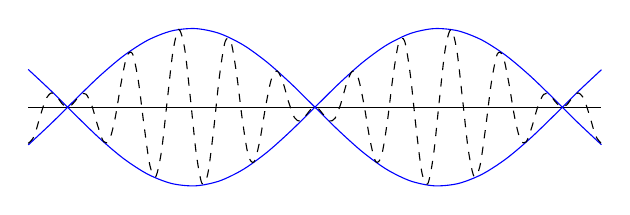
\begin{tikzpicture}
		\draw (-0.5,0) -- (6.78, 0);
		\draw[smooth,blue] plot[domain=-0.5:6.78] ({\x},{sin(deg(\x))});
		\draw[smooth,blue] plot[domain=-0.5:6.78] ({\x},{-sin(deg(\x))});
		\draw[smooth,dashed] plot[domain=-0.50:6.78,samples=100] ({\x},{sin(10*deg(\x))*sin(deg(\x))});
	\end{tikzpicture}
\end{center}

\subsubsection{Internal gravity wave velocities}
For internal gravity waves we have dispersion relation
\begin{equation}
	\frac{\omega^2}{N^2} = \frac{ k^2 + l^2}{k^2+l^2+m^2} = \cos^2 \theta
\end{equation}
Hence the phase velocity is
\begin{align}
	\symbf{c}_p = \frac{\omega}{\abs{\symbf{k}}^2}\symbf{k} 
	&= N
	\frac{(k^2+l^2)^{1/2}}{(k^2+l^2+m^2)^{3/2}}\symbf{k} \\
	&= \frac{N \cos\theta}{\abs{\symbf{k}}^2} \begin{pmatrix} \abs{\symbf{k}}
		\cos \varphi \cos \theta \\ \abs{\symbf{k}} \sin\varphi \cos\theta \\
	\abs{\symbf{k}} \sin\theta \end{pmatrix} \\
	&= \frac{ N \abs{\cos\theta}}{\abs{k}} \begin{pmatrix}
		\cos \varphi \cos \theta \\  \sin\varphi \cos\theta \\
	\sin\theta \end{pmatrix} \\
\end{align}
The prefactor is the magnitude of the phase velocity. The locus of possible
phase velocities for given $N$ and $\symbf{k}$ is two circles:
\begin{center}
	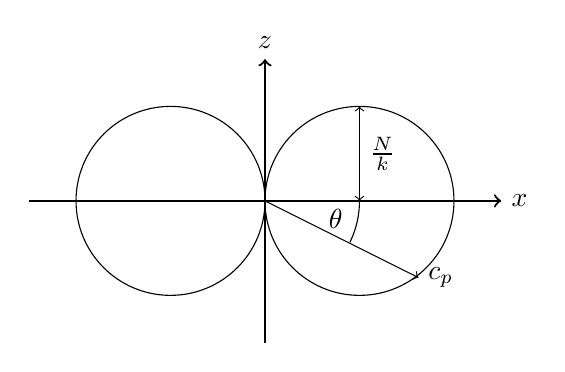
\begin{tikzpicture}[scale=1.5]
		\draw[thick,->] (-2, 0) -- (2, 0) node[right] {$x$};
		\draw[thick,->] (0, -1.2) -- (0, 1.2) node[above] {$z$};
		\draw (0.8, 0) circle (0.8);
		\draw (-0.8, 0) circle (0.8);
		\draw[->] (0,0) -- (1.3, -0.65) node[right] {$\symbf{c}_p$};
		\draw[<->] (0.8, 0) -- (0.8,0.8) node [midway,right] {$\frac{N}{\abs{\symbf{k}}}$};
		\draw (0.8,0) arc (0:-26:0.8);
		\draw (0.6, -0.15) node {$\theta$};
	\end{tikzpicture}
\end{center}

The group velocity is
\begin{equation}
	\symbf{c}_g = \frac{\partial \omega}{\partial \symbf{k}} =
	\frac{1}{2\omega} \frac{\partial \omega^2}{\partial \symbf{k}} =
	\frac{\omega}{\abs{\symbf{k}}^2} \left( \frac{N^2}{\omega^2} K\symbf{k} -
	m \symbf{\hat{z}}) - \symbf{k}\right) = \frac{N}{\abs{\symbf{k}}}
	\abs{\sin\theta} \begin{pmatrix} \cos \varphi \sin \theta \\ \sin \varphi
	\sin \theta \\ -\cos \theta \end{pmatrix}
\end{equation}
Hence the magnitude of the group velocity is $N
\abs{\sin\theta}/\abs{\symbf{k}}$. The group velocity is perpendicular to the
phase velocity:
\begin{center}
	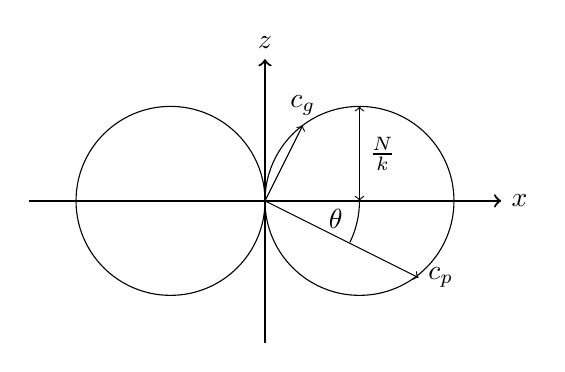
\begin{tikzpicture}[scale=1.5]
		\draw (0.8,0) arc (0:-26:0.8);
		\draw (0.6, -0.15) node {$\theta$};
		\draw[thick,->] (-2, 0) -- (2, 0) node[right] {$x$};
		\draw[thick,->] (0, -1.2) -- (0, 1.2) node[above] {$z$};
		\draw (0.8, 0) circle (0.8);
		\draw (-0.8, 0) circle (0.8);
		\draw[->] (0,0) -- (1.3, -0.65) node[right] {$\symbf{c}_p$};
		\draw[<->] (0.8, 0) -- (0.8,0.8) node [midway,right] {$\frac{N}{\abs{\symbf{k}}}$};
		\draw[->] (0,0) -- (0.32, 0.64) node[above] {$\symbf{c}_g$};
	\end{tikzpicture}
\end{center}

Note that 
\begin{equation}
	\symbf{c}_g + \symbf{c}_p = \frac{N}{\abs{\symbf{k}}} \left[
	\abs{\cos\theta} \begin{pmatrix} \cos\varphi \cos\theta \\
	\sin\varphi\cos\theta \\\sin\theta \end{pmatrix} + \abs{\sin\theta}
	\begin{pmatrix} \cos\varphi\sin\theta\\\sin\varphi\sin\theta \\
	-\cos\theta \end{pmatrix} \right] = \frac{N}{\abs{\symbf{k}}}
	\begin{pmatrix} \cos\varphi \\ \sin \varphi \\ 0 \end{pmatrix}
\end{equation}
Hence $\abs{\symbf{c}_p + \symbf{c}_g} = N/\abs{\symbf{k}}$ and $c_{pz} =
-c_{gz}$. Note also that $\symbf{c}_p \cdot \symbf{c}_g = 0$.

\subsection{Equipartition of energy}
We can form an energy equation from the momentum equation dotted with
$\symbf{u}$:
\begin{equation}
	\symbf{u} \cdot \left( \rho \frac{\partial \symbf{u}}{\partial t} + \rho
	(\symbf{u}\cdot\nabla)\symbf{u} + \nabla p + \rho g \hat{\symbf{z}}\right)
	= 0
\end{equation}
Using the Boussinesq approximation and linearising, we get
\begin{align}
	\symbf{u} \cdot \left( \rho_0 \frac{\partial \symbf{u}}{\partial t} +
	\nabla p' + \rho' g \hat{\symbf{z}}\right) &= 0 \\
	\frac{1}{2}\rho_0 \frac{\partial}{\partial t} \abs{\symbf{u}}^2 +
	\symbf{u} \cdot p' + w \rho' g &= 0
\end{align}
The first term is the rate of change of kinetic energy, the second is the work
against pressure gradients, and the last is the rate of change of potential
energy.

Using linearised conservation of mass we have
\begin{equation}
	\frac{\partial \rho'}{\partial t} + w \frac{\diffd \hat{\rho}}{\diffd z} =
	\frac{\partial \rho'}{\partial t} - w \frac{\rho_0}{g} N^2 = 0 \implies w
	= \frac{g}{\rho_0 N^2} \frac{\partial \rho'}{\partial t}
\end{equation}
Hence also using $\nabla \cdot \symbf{u} = 0$ we have the energy equation
\begin{equation}
	\frac{\partial}{\partial t} \left[ \frac{1}{2}\rho_0 \abs{\symbf{u}}^2 +
	\frac{1}{2}\frac{g^2}{\rho_0 N^2} \rho'^2 \right] + \nabla \cdot (p'
	\symbf{u}) = 0
\end{equation}
The term proportional to $\rho'^2$ is \emph{potential energy}. To see this,
consider a parcel of fluid raised vertically by some amount $\zeta$. The
buoyant force on the parcel is
\begin{equation} 
	F = V g \frac{\diffd \hat{\rho}}{\diffd z} (z-z_0)
\end{equation}
Hence the potential energy gained is
\begin{equation}
	\text{PE} = \int_{z_0}^{z_0 + \zeta} g \frac{\diffd \hat{\rho}}{\diffd z} (z-z_0)
	\, \diffd z = \frac{1}{2} \rho_0 N^2 \zeta^2
\end{equation}
Now from hydrostatic balance
\begin{equation}
	\rho' = -\frac{\diffd \hat{\rho}}{\diffd z} \zeta = \frac{\rho_0}{g}N^2
	\zeta
\end{equation}
Hence the potential energy can be written in the following equivalent ways
\begin{equation}
	\text{PE} = \frac{1}{2}\rho_0 N^2 \zeta^2 = \frac{1}{2}\frac{g^2}{\rho_0 N^2}
	\rho'^2 = \frac{1}{2}\rho_0 \frac{b^2}{N^2}
\end{equation}
So we have the energy equation
\begin{equation}
	\frac{\partial}{\partial t} \left[ \text{KE} + \text{PE}\right] + \nabla
	\cdot (p'\symbf{u}) = 0
\end{equation}
Integrating over a volume $V$ we have
\begin{equation}
	\int_V
	\frac{\partial}{\partial t} \left[ \text{KE} + \text{PE}\right] \diffd V
	+\int_S p'\symbf{u}\cdot\symbf{n}\,\diffd S = 0
\end{equation}
Define the flux of energy, or work against pressure, as $\symbf{F}_E =
p'\symbf{u}$. Recall that for a wave $\eta = \tilde{\eta}e^{i\phi}$, ,the
dynamical variables $u, w, b, p'$ can be expressed for $\tilde{\eta} \in
\mathbb{R}$ as
\begin{align}
	u &= \tilde{\eta} \omega \sin\theta \sin\phi \\
	w &= -\tilde{\eta} \omega \cos\theta \sin\phi \\
	b &= \tilde{\eta} \frac{\omega^2}{\cos^2 \theta} \\
	p' &= \tilde{\eta} \rho_0
	\frac{\omega^2}{\abs{\symbf{k}}}\tan\theta\sin\phi
\end{align}
Therefore we can write the KE and PE as
\begin{align}
	\text{KE} &= \frac{1}{2}\rho_0 (u^2 + w^2) = \frac{1}{2} \rho_0 \omega^2
	\tilde{\eta}^2 \sin^2 \phi \\
	\text{PE} &= \frac{1}{2}\rho_0 \omega^2 \tilde{\eta}^2 \cos^2\phi \\
	\implies \overline{\text{KE}} &= \overline{\text{PE}} = \frac{1}{4}\rho_0
	\omega^2 \tilde{\eta}^2
\end{align}
where $\overline{\cdot}$ denotes an average of a wavelength or period.
Equipartition of energy is the statement $\overline{E} = \overline{\text{KE}}
+ \overline{\text{PE}} = 2\overline{\text{KE}} = 2\overline{\text{PE}}$. We
may write the energy flux as
\begin{equation}
	\symbf{F}_E = p'\overline{u} = \rho_0 \omega^2 \tilde{\eta}^2 \sin^2 \phi
	\frac{N}{\abs{\symbf{k}}} \sin\theta \begin{pmatrix} \sin\theta \\ -\cos
	\theta \end{pmatrix}
\end{equation}
The average energy flux is then
\begin{equation}
	\overline{\symbf{F}_E}= \frac{1}{2}\rho_0 \omega^2 \tilde{\eta}^2
	\symbf{c}_g = \overline{E}\symbf{c}_g
\end{equation}
which is the average energy multipled by the group velocity, which justifies
the term `energy flux', and shows energy is transported with the group velocity.


\subsection{Amplitude decay along a beam}
Consider a point source which generates a beam of internal waves, in a 2D
incompressible fluid. We assume the buoyancy frequency $N$ is constant, and
set it equal to 1 for convenience. Also assume $\kappa = 0$, i.e. no
diffusion. The governing equations are
\begin{align}
	\nabla \cdot \symbf{u} &= 0 \\
	\frac{\partial u}{\partial t} + \frac{1}{\rho_0} \frac{\partial
\rho}{\partial x} &= \nu \nabla^2 u \\
\frac{\partial w}{\partial t} + \frac{1}{\rho_0} \frac{\partial p}{\partial z}
- b &= \nu \nabla^2 w \\
\frac{\partial b}{\partial t} + N^2 w &= 0 
\end{align}
where $b = - g \frac{\rho-\rho_0}{\rho_0}$. In 2D, we may introduce a
streamfunction $\symbf{\psi} = (0,\psi,0)$ so that
\begin{equation}
	\symbf{u} = \nabla \times \symbf{\psi} e^{-i\omega t} = (-\frac{\partial
	\psi}{\partial z}, 0, \frac{\partial \psi}{\partial x}) e^{-i\omega t}
\end{equation}
It is convenient to transform to a co-ordinate system $(\xi, \zeta)$ where
$\xi$ is in the direction of $\symbf{k}$ and $\zeta$ is in the direction of
$\symbf{c}_g$, i.e.
\begin{align}
	\xi &= x \cos \theta - z \sin \theta \\
	\zeta &= x \sin \theta + z \cos \theta 
\end{align}
In this co-ordinate system, the three governing equations can be reduced to two:
\begin{align}
	\frac{\partial b}{\partial t} + \frac{\partial \psi}{\partial \xi} \cos
	\theta + \frac{\partial \psi}{\partial \zeta} \sin \theta &= 0 \\
	-i\omega \left( \frac{\partial^2 \psi}{\partial \xi^2} + \frac{\partial^2
	\psi}{\partial \zeta^2}\right) - \frac{\partial b}{\partial \zeta} \sin
	\theta - \frac{\partial b}{\partial \xi} \cos \theta - \nu \nabla^4 \psi
															  &= 0 
\end{align}
Assuming the viscosity is small, we expand $b$ and $\psi$ in the small
parameter $\varepsilon = \nu/2$:
\begin{align}
	b &= (b_0 + \varepsilon b_1 + \dots) e^{-i\omega t} \\
	\psi &= (\psi_0 + \varepsilon \psi_1 + \dots )e^{-i\omega t}
\end{align}
Further we define a scaled coordinate $\chi = \varepsilon \zeta / \sin
\theta$. At order $\varepsilon^0$ we have:
\begin{align}
	\frac{\partial \psi_0}{\partial \xi} &= ib_0 \\
	\frac{\partial^2 \psi_0}{\partial \xi^2} &= i \frac{\partial b_0}{\partial
	\xi} 
\end{align}
At order $\varepsilon^1$:
\begin{align}
	\omega \frac{\partial \psi_1}{\partial \xi} - i \omega b_1 &= -
\frac{\partial \psi_0}{\partial \chi} \\
i\omega \frac{\partial^2 \psi_1}{\partial \xi^2} + \omega \frac{\partial
b_1}{\partial \xi} &= i \frac{\partial^2 \psi_0}{\partial \xi \partial \chi} -
2 \frac{\partial^4 \psi_0}{\partial \xi^4}
\end{align}
From these we form a governing equation for $\psi_0$:
\begin{equation}
	\frac{\partial^4 \psi_0}{\partial \xi^4} = i \frac{\partial^2
	\psi_0}{\partial \xi \partial \chi} \implies \frac{\partial^3
\psi_0}{\partial \xi^3} = i \frac{\partial \psi_0}{\partial \chi} + f(\chi)
\end{equation}
For a point source, as $\abs{\xi} \to \infty$, we except $\psi$ will tend to a
constant. Hence $f(\chi) \equiv 0$. The governing equation is separable:
suppose $\psi_0 = F(\xi) G(\chi)$. Then
\begin{align}
	\frac{F'''}{F} &= i \frac{G'}{G} = -ik^3 \\
	\implies G(\chi) &= e^{-k^3 \chi}, \hspace{1em} F(\xi) = e^{ik\xi}
\end{align}
The streamfunction is therefore $\psi = Ae^{-k^3 \chi} e^i\phi$. If $N$ is
constant but \emph{not} equal to 1, we have
\begin{align}
	\chi &= \frac{\nu}{2N\sin\theta}\zeta \\
	\implies \psi &= A \exp \left( \frac{-k^3 \nu \zeta}{2N\sin\theta}\right)
	e^{i\phi}
\end{align}
If $A$ depends on $k$ then
\begin{equation}
	\psi = \int_{-\infty}^\infty A(k) e^{-i\omega t} \exp \left( ik\xi -
	\frac{\nu k^3}{2N\sin\theta} \zeta \right) \, \diffd k
\end{equation}
In the case of an oscillating cylinder, the beams are well described by point
sources at the tangent points on the cylinder, and from above the amplitude is
initially bimodal but smooths out (decays) to become unimodal:
\begin{center}
	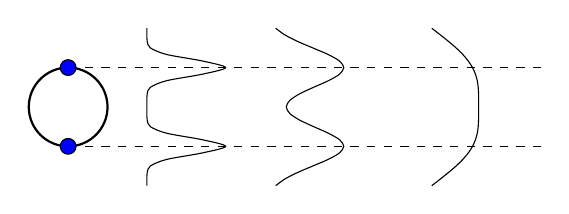
\begin{tikzpicture}
		\draw[thick] (0,0) circle (0.5);
		\draw[dashed] (0, 0.5) -- (6, 0.5);
		\draw[dashed] (0, -0.5) -- (6, -0.5);
		\draw[fill=blue] (0,0.5) circle (0.1);
		\draw[fill=blue] (0,-0.5) circle (0.1);
		\draw[smooth] plot[domain=-1:1] ({1+exp(-50*(\x-0.5)^2) +
		exp(-50*(\x+0.5)^2)},{\x});
		\draw[smooth] plot[domain=-1:1] ({2.5+exp(-8*(\x-0.5)^2) +
		exp(-8*(\x+0.5)^2)},{\x});
		\draw[smooth] plot[domain=-1:1] ({4+exp(-2*(\x-0.5)^2) +
		exp(-2*(\x+0.5)^2)},{\x});
	\end{tikzpicture}
\end{center}
We can form a Reynolds number to characterise these waves. Recall
$\abs{\symbf{c}_g} = N\sin\theta / \abs{\symbf{k}}$. Hence
\begin{equation}
	-\frac{\nu k^3}{2N\sin\theta} \zeta = - \frac{\nu k}{2}
	\frac{k}{N\sin\theta} k \zeta = - \pi \frac{\nu}{\lambda
	\abs{\symbf{c}_g}} k \zeta = - \pi \text{Re}^{-1} k \zeta
\end{equation}
where $\lambda = 2\pi/k$ is the wavelength. Thus we have
\begin{equation}
	\text{Re} = \frac{\lambda \abs{\symbf{c}_g}}{\nu}
\end{equation}
in analogy with the usual definition of Reynolds number, $UL/\nu$.

\subsection{Mass diffusivity}
In some situations, the fluid mass may diffuse, in which case mass
conservation is modified to
\begin{equation}
	\frac{\diffD \rho}{\diffD t} = \kappa \nabla^2 \rho
\end{equation}
If $\rho = \rho(S, T, \phi)$ then
\begin{equation}
	\frac{\diffD S}{\diffD t} = \kappa_S \nabla^2 S, \hspace{2em} \frac{\diffD
	T}{\diffD t} = \kappa_T \nabla^2 T
\end{equation}
The ratio of viscosity to thermal diffusivity is characterised by the
\emph{Prandtl number} $\text{Pr} = \nu/\kappa_T$. For heat diffusion in air,
$\text{Pr} \sim 0.7$ and in water, $\text{Pr} \sim 7$. A more general
\emph{Schmidt number} $\text{Sc} = \nu/\kappa_S$ characterises viscosity
versus diffusion of some concentration, e.g. salt. Salt in water has
$\text{Sc} \sim 700$. 

\subsection{Reflections of waves}
\subsubsection{Properties of beams}
For simplicity, assume $N^2$ constant. The usual laws of optics imply the
incident angle is equal to the reflection angle. Thus $\omega/N = \cos\theta$
is conserved, assuming no Doppler shift, i.e. the boundary is stationary. 

\begin{center}
	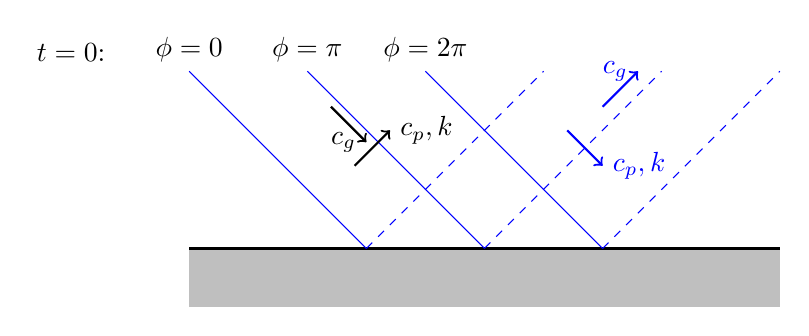
\begin{tikzpicture}[scale=1.5]
		\draw[fill=gray!50, draw=none] (0,0) rectangle (5, -0.5);
		\draw[thick] (0,0) -- (5, 0);
		\draw[blue] (0, 1.5) -- (1.5, 0);
		\draw[blue,dashed] (1.5, 0) -- (3, 1.5);
		\draw[blue] (1, 1.5) -- (2.5, 0);
		\draw[blue,dashed] (2.5, 0) -- (4, 1.5);
		\draw[blue] (2, 1.5) -- (3.5, 0);
		\draw[blue,dashed] (3.5, 0) -- (5, 1.5);
		\draw (0, 1.5) node[above] {$\phi = 0$};
		\draw (1, 1.5) node[above] {$\phi = \pi$};
		\draw (2, 1.5) node[above] {$\phi = 2\pi$};
		\draw (-1, 1.5) node[above] {$t=0$:};
		\draw[thick,->] (1.2, 1.2) -- ++(0.3,-0.3) node[left] {$\symbf{c}_g$};
		\draw[thick,->] (1.4, 0.7) -- ++(0.3,0.3) node[right] {$\symbf{c}_p,
		\symbf{k}$};
		\draw[blue,thick,->] (3.5, 1.2) -- ++(0.3,0.3) node[left]
		{$\symbf{c}_g$};
		\draw[blue,thick,->] (3.2, 1) -- ++(0.3, -0.3) node[right]
		{$\symbf{c}_p, \symbf{k}$};
	\end{tikzpicture}
\end{center}

In the case of a horizontal reflection boundary, the vertical component of
$\symbf{u}$ is reversed, whilst the horizontal component is preserved. Energy
conservation implies the magnitude of the flux of energy $\overline{\symbf{F}} =
\overline{E}\symbf{c}_g$ is conserved, i.e. $\abs{\overline{\symbf{F}}_i} =
\abs{\overline{\symbf{F}}_r}$. We also have wavelength conserved, $\lambda_i =
\lambda_r$, wavevector magnitude conserved, $\abs{\symbf{k}_i} =
\abs{\symbf{k}_r}$, and group velocity magnitude conserved,
$\abs{\symbf{c}_{gi}} = \abs{\symbf{c}_{gr}}$. Consequently, the wave energy
$\overline{E}_i = \overline{E}_r$ is conserved.

In the case of a vertical reflection boundary, the energy flux remains
conserved, but instead the vertical component of $\symbf{u}$ is reversed and
the vertical component is preserved.

\begin{center}
	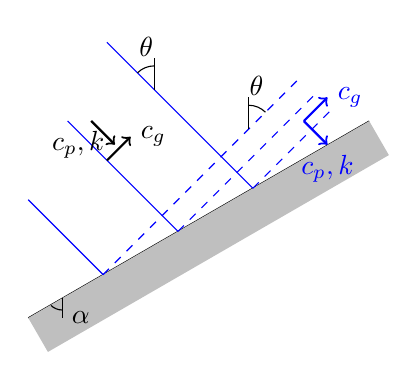
\begin{tikzpicture}
		\draw(0,0) -- (4.33,2.5);
		\draw[draw=none,fill=gray!50,rotate=30] (0,0) rectangle (5, -0.5);
		\draw[blue] (0, 1.5) -- (0.951, 0.549);
		\draw[blue,dashed] (0.951, 0.549) -- ++ (2.5, 2.5);
		\draw[blue] (0.5, 2.5) -- (1.902, 1.098);
		\draw[blue,dashed] (1.902, 1.098) -- ++ (1.75, 1.75);
		\draw[blue] (1, 3.5) -- (2.853, 1.647);
		\draw[blue,dashed] (2.853, 1.647) -- ++ (1, 1);

		\draw (1.6, 2.9) -- (1.6, 3.3);
		\draw (1.6, 3.2) arc (90:135:0.3);
		\draw (1.5, 3.2) node[above] {$\theta$};

		\draw (2.8, 2.4) -- (2.8, 2.8);
		\draw (2.8, 2.7) arc (90:45:0.3);
		\draw (2.9, 2.7) node[above] {$\theta$};

		\draw[thick,->] (0.8, 2.5) -- ++ (0.3,-0.3) node[left] {$\symbf{c}_p,
		\symbf{k}$};
		\draw[thick,->] (1, 2) -- ++ (0.3, 0.3) node[right] {$\symbf{c}_g$};

		\draw[blue,thick,->] (3.5, 2.5) -- ++ (0.3,0.3) node[right]
		{$\symbf{c}_g$};
		\draw[blue,thick,->] (3.5, 2.5) -- ++ (0.3, -0.3) node[below]
		{$\symbf{c}_p, \symbf{k}$};

		\draw (0.43, 0.25) -- (0.43, 0);
		\draw (0.43, 0.1) arc (-90:-135:0.2);
		\draw (0.43, 0) node[right] {$\alpha$};
	\end{tikzpicture}
\end{center}

Finally, with a boundary at some angle $\alpha$ to the vertical, since
$\theta$ is determined by the dispersion relation it is still conserved after
reflection. Waves also preserve frequency, since it is set by the source, so
$\theta_i = \theta_r$ and $\omega_i = \omega_r$. The wave displacement
satisfies
\begin{equation}
	\abs{\tilde{\eta}_r} = \gamma \abs{\tilde{\eta}_i}
\end{equation}
where the magnitude is scaled by
\begin{equation}
	\gamma = \abs{\frac{\sin(\theta+\alpha)}{\sin(\theta-\alpha)}} > 1
\end{equation}

\subsubsection{Energy density upon reflection}
For reflection from a boundary at general angle $\alpha$, we have scalings
\begin{align}
	\abs{\symbf{k}_r} &= \gamma \abs{\symbf{k}_i} \iff \lambda_r =
		\frac{1}{\gamma} \lambda_i \\
	\abs{\tilde{w}_r} &= \gamma \abs{\tilde{w}_i} \\
	\abs{\tilde{\eta}_r} &= \gamma \abs{\tilde{\eta}_i} \\
	\abs{\symbf{c}_{gr}} &= \frac{1}{\gamma} \abs{\symbf{c}_{gi}}\\
	\abs{\tilde{\symbf{F}}_r} &= \abs{\tilde{\symbf{F}}_i}
\end{align}
where $\tilde{\symbf{F}}$ is the energy flux per unit wavelength. The energy
density per unit wavelength is
\begin{equation}
	\tilde{E} = \int_0^\lambda \text{PE} + \text{KE} \, \diffd \xi
\end{equation}
with $\tilde{\symbf{F}} = \tilde{E} \symbf{c}_g$ and hence $\tilde{E}_r =
\gamma \tilde{E}_i$, since
\begin{equation}
	\tilde{E} \sim \lambda (\text{PE} + \text{KE}) \sim \lambda
	(\abs{\tilde{\eta}}^2 + \abs{\tilde{w}}^2)
\end{equation}
and $\lambda$ scales by $1/\gamma$, whilst the terms in the bracket scale as
$\gamma^2$. 

The energy density per unit \emph{length} is instead
\begin{equation}
	\hat{E} = \frac{1}{\lambda} \int_0^\lambda \text{PE} + \text{KE} \, \diffd
	\xi = \frac{1}{\lambda} \tilde{E}
\end{equation}
Hence $\tilde{\symbf{F}} = \lambda \hat{E} \symbf{c}_g$. The flux of energy
per unit wavelength is conserved, so
\begin{equation}
	\lambda_r \hat{E}_r \abs{\symbf{c}_{gr}} = \frac{1}{\gamma} \lambda_i
	\hat{E}_r \frac{1}{\gamma} \abs{\symbf{g}_{gi}} = \lambda_i \hat{E}_i
	\abs{\symbf{c}_{gi}}
\end{equation}
Hence $\hat{E}_r = \gamma^2 \hat{E}_i$. Denote the lengthscale for wave crests
as $L_i$ for the incident wave and $L_r$ for the reflected wave. The total
energy is then
\begin{align}
	\text{TE}_r &= \int_{-\infty}^\infty \text{PE}_r + \text{KE}_r \, \diffd
	\xi \\
				&= \int_{-L_r/2}^{L_r/2} \text{PE}_r + \text{KE}_r \, \diffd
				\xi \\
				&= \gamma^2 \int_{-L_i/2\gamma}^{L_i/2\gamma}
				\text{PE}_i+\text{KE}_i \, \diffd \xi \\
				&= \gamma T E_i
\end{align}
Spectral energy denity $S(k)$ obeys
\begin{equation}
	S_r(k) = \gamma S_i(k/\gamma)
\end{equation}

\subsubsection{Critical reflections}
Subcritical reflections are where the vertical component of the group velocity
reverses, whilst supercritical reflections are those where the horizontal
component of the group velocity reverses. 

\begin{center}
	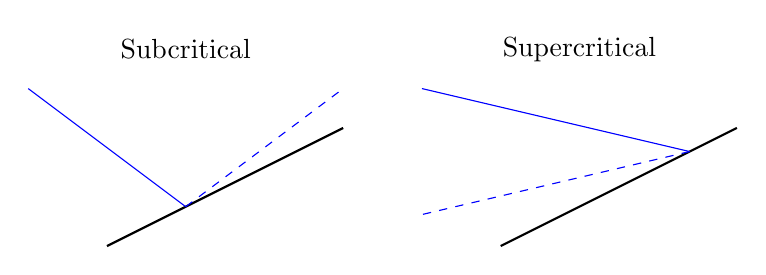
\begin{tikzpicture}
		\draw (1, 2.5) node {Subcritical};
		\draw[thick] (0,0) -- (3, 1.5);
		\draw[blue] (-1, 2) -- (1, 0.5);
		\draw[blue,dashed] (1, 0.5) -- (3, 2);
		\begin{scope}[shift={(5, 0)}]
			\draw (1, 2.5) node {Supercritical};
			\draw[thick] (0,0) -- (3, 1.5);
			\draw[blue] (-1, 2) -- (2.4, 1.2);
			\draw[blue,dashed] (2.4, 1.2) -- (-1, 0.4);
		\end{scope}
	\end{tikzpicture}
\end{center}

At critical slope $\theta = \alpha$,
$\gamma \to \infty$.  If $\lambda \to \infty$ then $\abs{\symbf{k}_r} \to
\infty$, $\abs{\tilde{\eta}_r} \to \infty$ and $\abs{\symbf{c}_{gr}} \to
0$. As usual, $\omega_r = \omega_i$. Linear incident waves become non-linear
after reflection close to criticality. The $e^{-\frac{\nu k^3 \zeta}{2N \sin
\theta}}$ decay of an internal wave beam, combined with amplification of the
wavenumber upon reflection and the no-slip boundary creates very rapid
dissipation of energy, and hence very strong non-linearities.

\subsubsection{Ray tracing}
In 2D, internal waves satisfy the wave equation
\begin{equation}
	\left(\nabla^2 \partial_t^2 + N^2 \nabla_H^2\right) \psi = 0
\end{equation}
where $\psi = \tilde{\psi}(x,z)e^{-i\omega t}$ is the streamfunction. We have
\begin{equation}
	(N^2 - \omega^2) \frac{\partial^2 \tilde{\psi}}{\partial x^2} - \omega^2
	\frac{\partial^2 \tilde{\psi}}{\partial z^2} = 0
\end{equation}
Define $\Lambda^2 = \omega^2 / (N^2-\omega)^2$. Then we have the
\emph{Poincar\'{e} wave equation}
\begin{equation}
	\left( \frac{\partial^2}{\partial x^2} - \Lambda^2
	\frac{\partial^2}{\partial z^2}\right) \tilde{\psi} = 0
\end{equation}

If the domain is bounded, $\tilde{\psi} = 0$ on the boundary but this is an
ill-posed problem. Instead, we use ray tracing which effectively follows the
energy around the domain. Consider a top-boundary with a sloping boundary
below it:
\begin{center}
	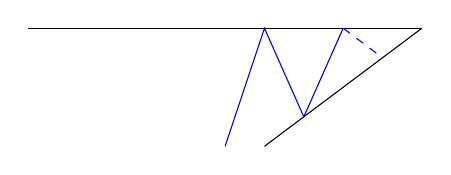
\begin{tikzpicture}
		\draw (0, 3) -- (5, 3);
		\draw (3, 1.5) -- (5, 3);
		\draw[blue] (2.5, 1.5) -- (3, 3) -- (3.5, 1.875) -- (4, 3);
		\draw[blue,dashed] (4,3) -- (4.5, 2.625);
	\end{tikzpicture}
\end{center}
The energy is trapped into the corner by repeated focusing reflections. For
large $\text{Re} = \abs{\symbf{c}_g}{\abs{\symbf{k}}\nu}$ then non-linearities
will dominate and possible breaking giving mixing. 

\subsubsection{Reflections from rough topography}
An incident monochromatic internal wave reflecting from a rough topography
will in general become a beam with a spectrum of wavenumbers, i.e.
$\symbf{k}_r$ is a spectrum. Consider for aexample a sine wave topography of
\emph{small amplitude}. We may then linearise the topography.








\end{document}
